Since early 2020, the CoViD-19 pandemic has presented an enormous challenge to humanity
on many dimensions. The development of highly effective vaccines holds the promise of
containment in the medium term. However, most countries find themselves many
months---and often years---away from reaching vaccination levels that would end the
pandemic or even protect the most vulnerable \citep{Mathieu2021}. In the meantime, it is
of utmost importance to employ an effective mix of strategies for containing the virus.
The most frequent initial response was a set of non-pharmaceutical interventions (NPIs)
to reduce contacts between individuals. While this has allowed some countries to sustain
equilibria with very low infection numbers,\footnote{See \citet{Contreras2021} for a
    theoretical equilibrium at low case numbers which is sustained with
    test-trace-and-isolate policies.} most have seen large fluctuations of infection rates
over time. Containment measures have become increasingly diverse and now include rapid
testing, more nuanced NPIs, and contact tracing. Neither these policies' effects nor the
influence of seasonal patterns or of more infectious virus strains are well understood
in quantitative terms.

This paper develops a quantitative model incorporating these factors simultaneously. The
framework allows to combine a wide variety of data and mechanisms in a timely fashion,
making it useful to predict the effects of various interventions. Behavioral reactions
to symptoms or positive tests are explicitly taken into account. We apply the model to
Germany, where new infections fell by almost 80\% during May 2021. Our analysis shows
that, aside from seasonality, frequent and large-scale rapid testing caused the bulk of
this decrease, which is in line with prior predictions \citep{Mina2021}. We conclude
that it should have a large role for at least as long as vaccinations have not been
offered to an entire population.

\section{Model description}

At the core of our agent-based model \citep[][we review more literature in Supplementary
    Material~\ref{sec:literature_review}]{Aleta2020,Hinch2021a} are physical contacts
between heterogeneous agents (Figure~\ref{fig:model_contacts_infections}). Each
contact between an infectious individual and somebody susceptible to the disease
bears the risk of transmitting the virus. Contacts occur in up to four networks:
Within the household, at work, at school, or in other settings (leisure activities,
grocery shopping, medical appointments, etc.). Some contacts recur regularly, others
occur at random. Empirical applications can take the population and household
structure from census data and the network-specific frequencies of contacts from
diary data measuring contacts before the pandemic
\citep[e.g.][]{Mossong2008,Hoang2019}. Within each network, meeting frequencies
depend on age and geographical location (see Supplementary
Material~\ref{subsec:assortativity}).

The four contact networks are chosen so that the most common NPIs can be modeled in
great detail. NPIs affect the number of contacts or the risk of transmitting the disease
upon having physical contact. The effect of different NPIs will generally vary across
contact types. For example, a mandate to work from home will reduce the number of work
contacts to zero for a fraction of the working population. Schools and daycare can be
closed entirely, operate at reduced capacity---including an alternating schedule---, or
implement mitigation measures like masking requirements or air filters
\citep{Lessler2021}. Curfews may reduce the number of contacts in settings outside of
work and school. In any setting, measures like masking requirements would reduce the
probability of infection associated with a contact \citep{Cheng2021}.

\begin{figure}   % Figure 1
    \centering

    \begin{subfigure}[b]{0.425\textwidth}
        \centering
        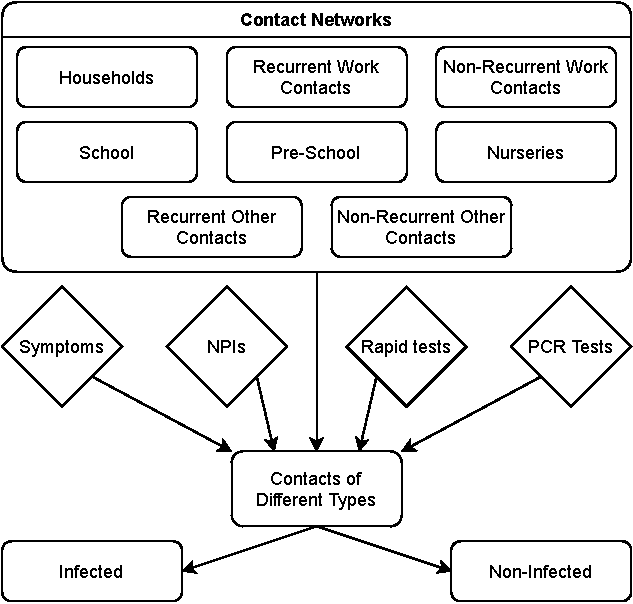
\includegraphics[width=\textwidth]{figures/model-graph-top-left}
        \caption{{Model for contacts and infections}}
        \label{fig:model_contacts_infections}
    \end{subfigure}
    \hfill
    \begin{subfigure}[b]{0.425\textwidth}
        \centering
        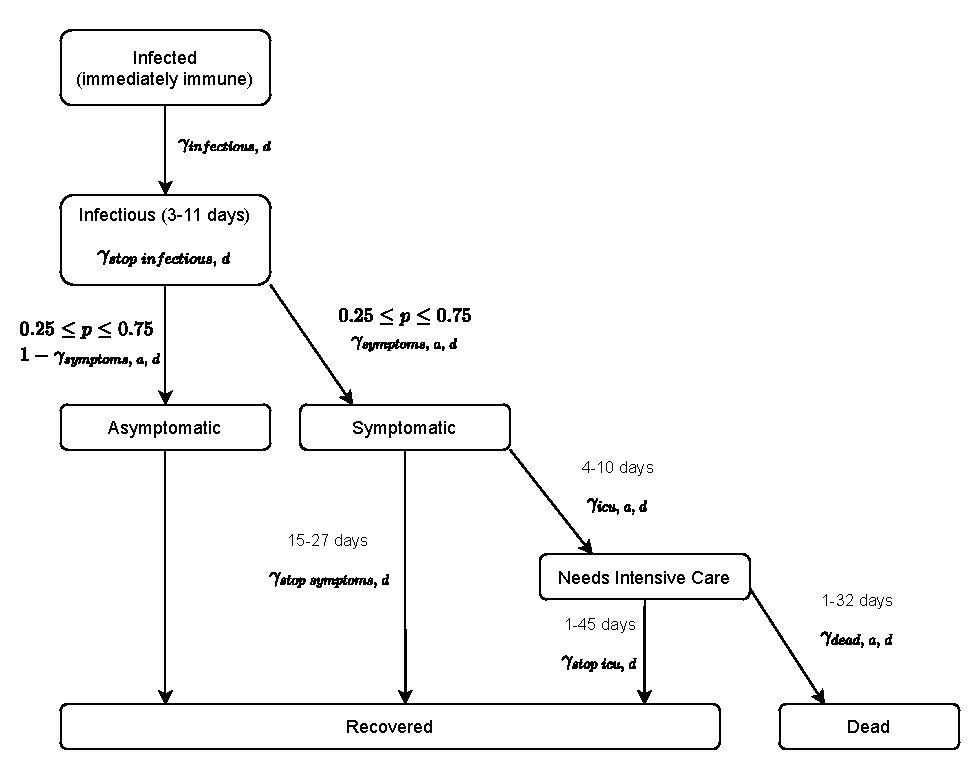
\includegraphics[width=\textwidth]{figures/model-graph-top-right}
        \vskip5ex

        \caption{Disease progression}
        \label{fig:model_disease_progression}
    \end{subfigure}
    \vskip3ex
    \begin{subfigure}[b]{0.425\textwidth}
        \centering

        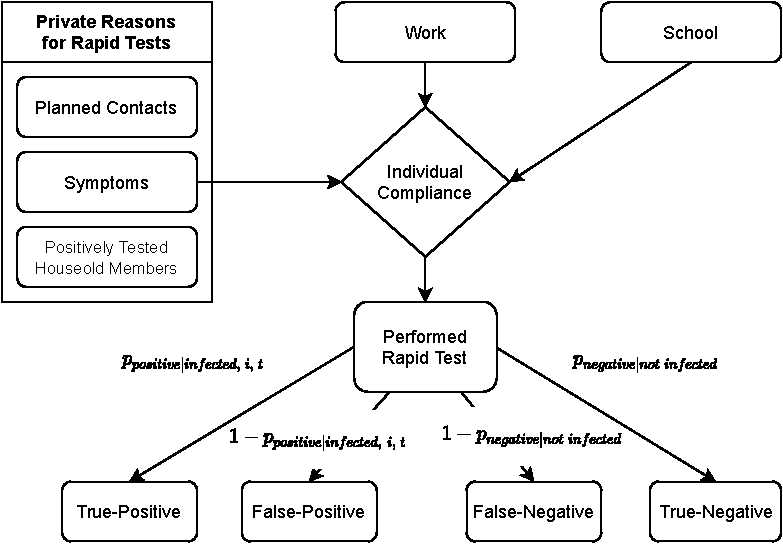
\includegraphics[width=\textwidth]{figures/model-graph-bottom-left}
        \caption{{Model for rapid tests}}
        \label{fig:model_rapid_tests}
    \end{subfigure}
    \hfill
    \begin{subfigure}[b]{0.425\textwidth}
        \centering
        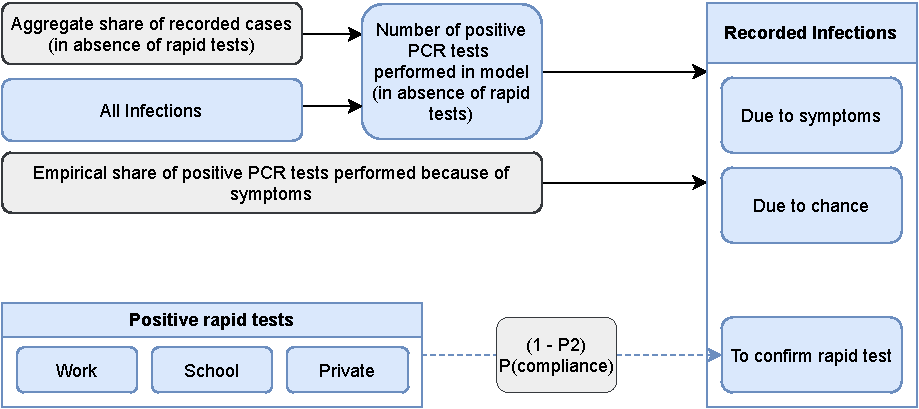
\includegraphics[width=\textwidth]{figures/model-graph-bottom-right}
        \vskip5ex

        \caption{{Translating all infections to recorded ones}}
        \label{fig:model_official_cases}
    \end{subfigure}

    \caption{Model description}
    \label{fig:model_description}

    \floatfoot{\noindent \textit{Note:}
        A~description of the model can be found in Supplementary
        Material~\ref{sec:supplementary_text}.
        Figure~\ref{fig:model_contacts_infections} shows the influence of an agent's
        contacts to other agents on infections. Demographic characteristics set the
        baseline number of contacts in different networks ($\eta$). The agents may
        reduce the number of contacts due to NPIs, showing symptoms, or testing
        positively for SARS-CoV-2 ($\tau$). Infections may occur when a susceptible
        agent meets an infectious agent; the probability depends on the type of contact
        ($\beta_c$), on seasonality ($\kappa_{c}$), and on NPIs ($\rho_{c,\:t}$). If
        infected, the infection progresses as depicted in
        Figure~\ref{fig:model_disease_progression}. If rapid tests are available,
        agents' demand is modeled as in Figure~\ref{fig:model_rapid_tests}. All reasons
        trigger a test only for a fraction of individuals depending on an individual
        compliance parameter; the thresholds for triggering test demand differ across
        reasons and they may depend on calendar time ($\pi_{c,\:t}$ and $\tau_{c,\:t}$).
        Figure~\ref{fig:model_official_cases} shows the model of translating all
        infections in the simulated data to age-specific recorded infections. The model
        uses data on the aggregate share of recorded cases ($\psi$), the share of
        positive PCR tests triggered by symptoms ($\chi_{symptom}$), and the false
        positive rate of rapid tests ($p_{positive|infected,\;i,\:t}$). The lower part
        of the graph is relevant only for periods where rapid tests are available. All
        parameters are explained in Appendix~\ref{sub:param_tables}.}
\end{figure}

In the model, susceptibility to contracting the SARS-CoV-2 virus is dependent on age
\citep{Davies2020,Goldstein2021}.\label{r.2.b} A possible infection progresses as shown
in Figure~\ref{fig:model_disease_progression}. We differentiate between an initial
period of infection without being infectious or showing symptoms, being infectious
(presymptomatic or asymptomatic), showing symptoms, requiring intensive care, and
recovery or death \citep[similar to][]{Aleta2020}. The probabilities of transitioning
between these states depend on age; their duration is random and calibrated to medical
literature (for a detailed description see Supplementary
Material~\ref{sub:data_course_of_disease}). Conditional on the type of contact,
infectiousness is independent of age \citep{Jones2021}.

The model includes several other features, which are crucial to describe the evolution
of the pandemic in 2020-2021. New virus strains with different infectiousness profiles
may appear. Vaccines may become available. During the vaccine roll-out, priority may
depend on age and occupation; vaccine hesitancy is modelled by some individuals refusing
vaccination offers. With some probability, vaccinated agents become immune and do not
transmit the virus \citep{Hunter2021, LevineTiefenbrun2021, Petter2021, Pritchard2021}.

We include two types of tests. Polymerase chain reaction (PCR) tests reveal whether an
individual is infected or not; there is no uncertainty to the result. PCR tests require
at least one day to be processed and there are aggregate capacity constraints. In
contrast, rapid antigen tests yield immediate results.
\label{r.1.a}\Copy{r.1.a}{Specificity and sensitivity of these tests is set according to
    data analyzed in \citet{Bruemmer2021,Scheiblauer2021,Özcürümez2021}; sensitivity depends
    on the timing of the test relative to the onset of infectiousness as in
    \citet{Smith2021}. We analyse robustness to different assumptions in
    Appendix~\ref{subsec:robustness_rapid_test_sensitivity}.} After a phase-in period, all
tests that are demanded will be performed. Figure~\ref{fig:model_rapid_tests} shows our
model for rapid test demand. Schools may require staff and students to be tested
regularly. Rapid tests may be offered by employers to on-site workers. Individuals may
demand tests for private reasons, which include having plans to meet other people,
showing symptoms of CoViD-19, and a household member having tested positively for the
virus. We endow each agent with an individual compliance parameter. This parameter
determines whether she takes up rapid tests.\footnote{Positive test results or symptoms
    lead most individuals to reduce their contacts; this is why tests impact the actual
    contacts in Figure~\ref{fig:model_description}.}

Modelling a population of agents according to actual demographic characteristics means
that we can use a wide array of data to identify and calibrate the model's many
parameters.\footnote{See Supplementary Material~\ref{sec:materials_and_methods} for a
    complete description.} Contact diaries yield pre-pandemic distributions of contacts for
different contact types and their assortativity by age group. Mobility data is used to
model the evolution of work contacts. School and daycare policies can be incorporated
directly from official directives. Administrative records on the number of tests,
vaccinations by age and region, and the prevalence of virus strains are generally
available. Surveys may ask about test offers, propensities to take them up, and past
tests. Other studies' estimates of the seasonality of infections can be incorporated
directly. The remaining parameters---most notably, these include infection probabilities
by contact network and the effects of some NPIs, see Supplementary
Material~\ref{subsec:estimated_params}---will be chosen numerically so that the model
matches features of the data \citep[see][for the general method]{McFadden1989}. In our
application, we keep the number of free parameters low in order to avoid overfitting.
The data features to be matched include official case numbers for each age group and
region, deaths, and the share of the B.1.1.7 strain.

The main issue with official case numbers is that they will contain only a fraction of
all infections. In the German case, this specifically amounts to positive PCR tests. We
thus model recorded cases as depicted in Figure~\ref{fig:model_official_cases}. We take
mortality-based aggregate estimates of the share of detected cases and use data on the
share of PCR tests administered because of CoViD-19 symptoms. As the share of
asymptomatic individuals varies by age group, this gives us age-specific shares (see
Figure~\ref{fig:share_known_cases_by_age_group}). Our estimates suggest that---in the
absence of rapid testing---the detection rate is 80\% higher on average for individuals
above age 80 compared to school age children. Once rapid test become available,
confirmation of a positive result is another reason leading to positive PCR tests.

\section{Second and third waves of the CoViD-19 pandemic in Germany}

The model is applied to the second and third waves of the CoViD-19 pandemic in Germany,
covering the period mid-September 2020 to the end of May 2021.
Figure~\ref{fig:pandemic_drivers_model_fit} describes the evolution of the pandemic and
of its drivers. The black line in Figure~\ref{fig:aggregated_fit} shows officially
recorded cases; the black line in Figure~\ref{fig:stringency_infectious_contacts} the
Oxford Response Stringency Index \citep{Hale2020}, which tracks the tightness of
non-pharmaceutical interventions. The index is shown for illustration of the NPIs, we
never use it directly. For legibility reasons, we transform the index so that lower
values represent higher levels of restrictions. A value of zero means all measures
incorporated in the index are turned on. The value one represents the situation in
mid-September, with restrictions on gatherings and public events, masking requirements,
but open schools and workplaces. In the seven weeks between mid September and early
November, cases increased by a factor of ten. Restrictions were somewhat tightened in
mid-October and again in early November. New infections remained constant throughout
November before rising again in December, prompting the most stringent lockdown to this
date. Schools and daycare centers were closed, so were customer-facing businesses except
for grocery and drug stores. From the peak of the second wave just before Christmas
until the trough in mid-February, newly detected cases decreased by almost three
quarters. The third wave in the spring of 2021 is associated with the B.1.1.7 (Alpha)
strain, which became dominant in March (Figure~\ref{fig:share_b117}).\footnote{B.1.617.2
    (Delta) was first detected in Germany in April; at the end of our simulation period it
    accounted for less than 5\% of cases.} In early March, some NPIs were relaxed; e.g.,
hairdressers and home improvement stores were allowed to open again to the public. There
were many changes in details of regulations afterwards, but they did not change the
overall stringency index.

\begin{figure}[!tp]   % Figure 2
    \centering

    \begin{subfigure}[b]{0.475\textwidth}
        \centering
        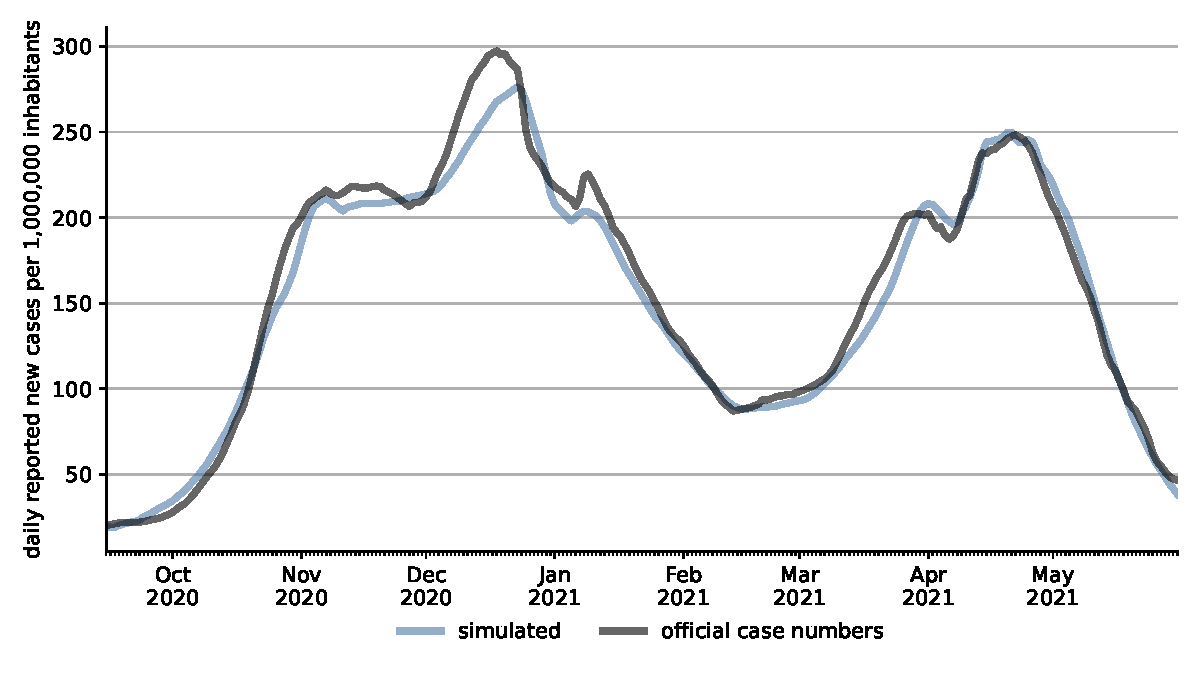
\includegraphics[width=\textwidth]{figures/results/figures/scenario_comparisons/combined_fit/full_new_known_case}
        \caption{{Recorded cases: Empirical and simulated}}
        \label{fig:aggregated_fit}
    \end{subfigure}
    \hfill
    \begin{subfigure}[b]{0.475\textwidth}
        \centering
        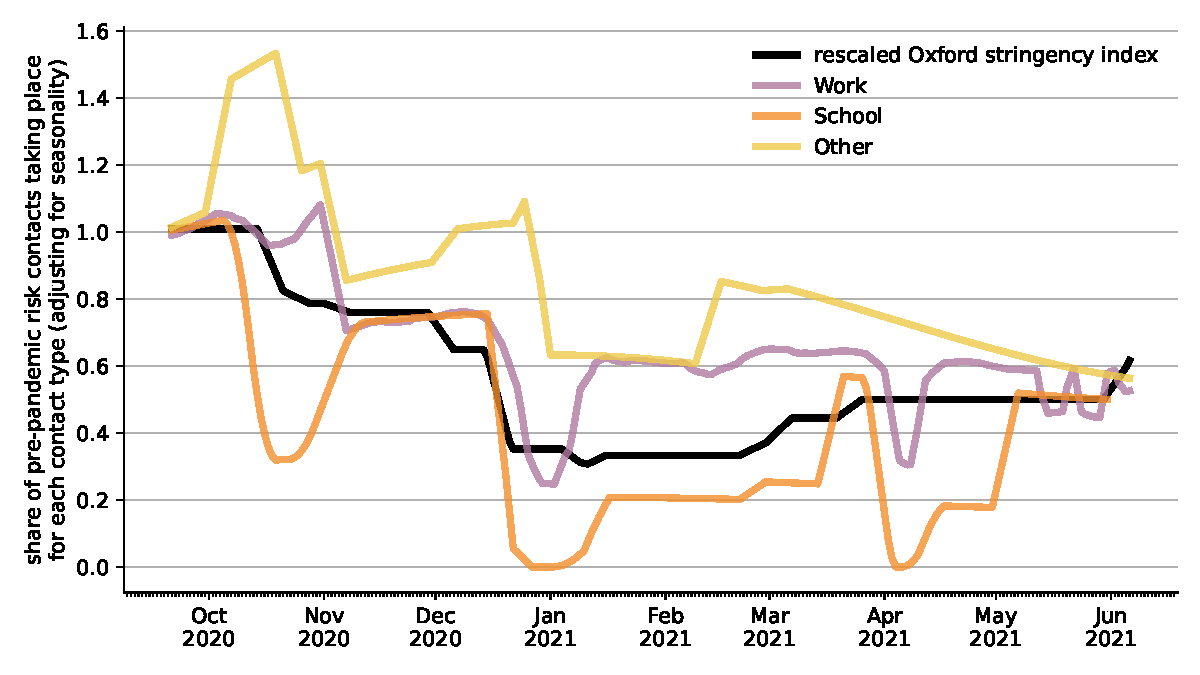
\includegraphics[width=\textwidth]{figures/results/figures/data/stringency2_with_seasonality}

        \caption{{Stringency of NPIs and infectious contacts}}
        \label{fig:stringency_infectious_contacts}
    \end{subfigure}

    \vskip3ex

    \begin{subfigure}[b]{0.475\textwidth}
        \centering

        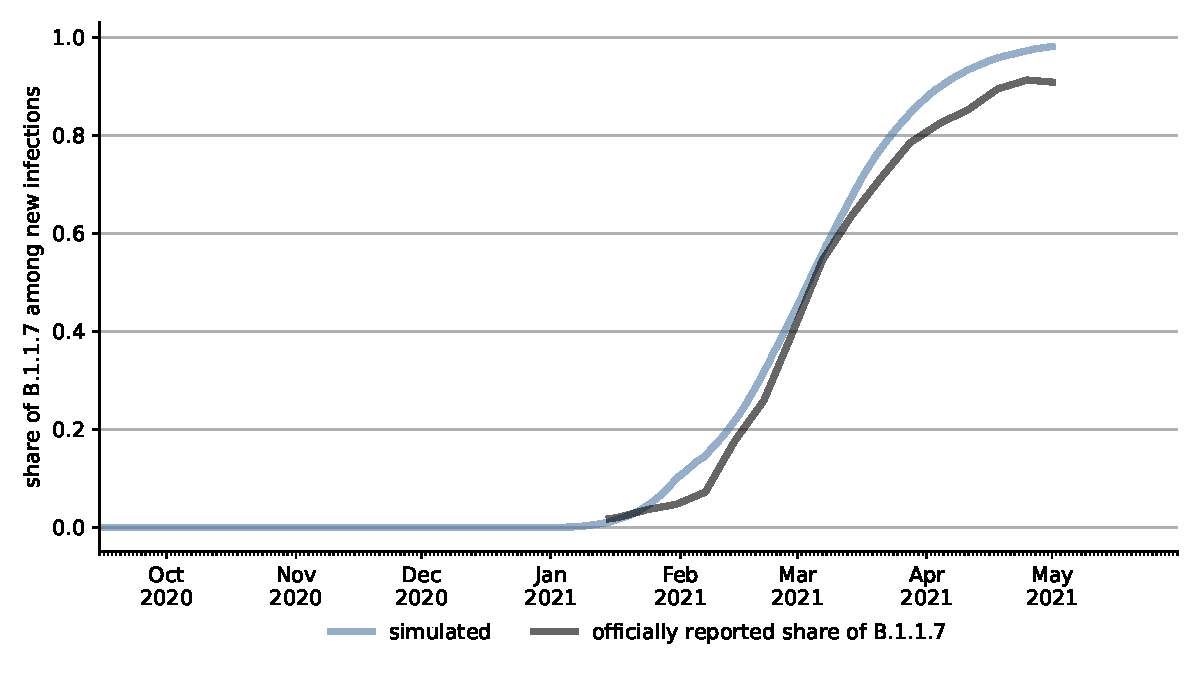
\includegraphics[width=\textwidth]{figures/results/figures/scenario_comparisons/combined_fit/full_share_b117}

        \caption{Fraction of B.1.1.7 strain}
        \label{fig:share_b117}
    \end{subfigure}
    \hfill
    \begin{subfigure}[b]{0.475\textwidth}
        \centering

        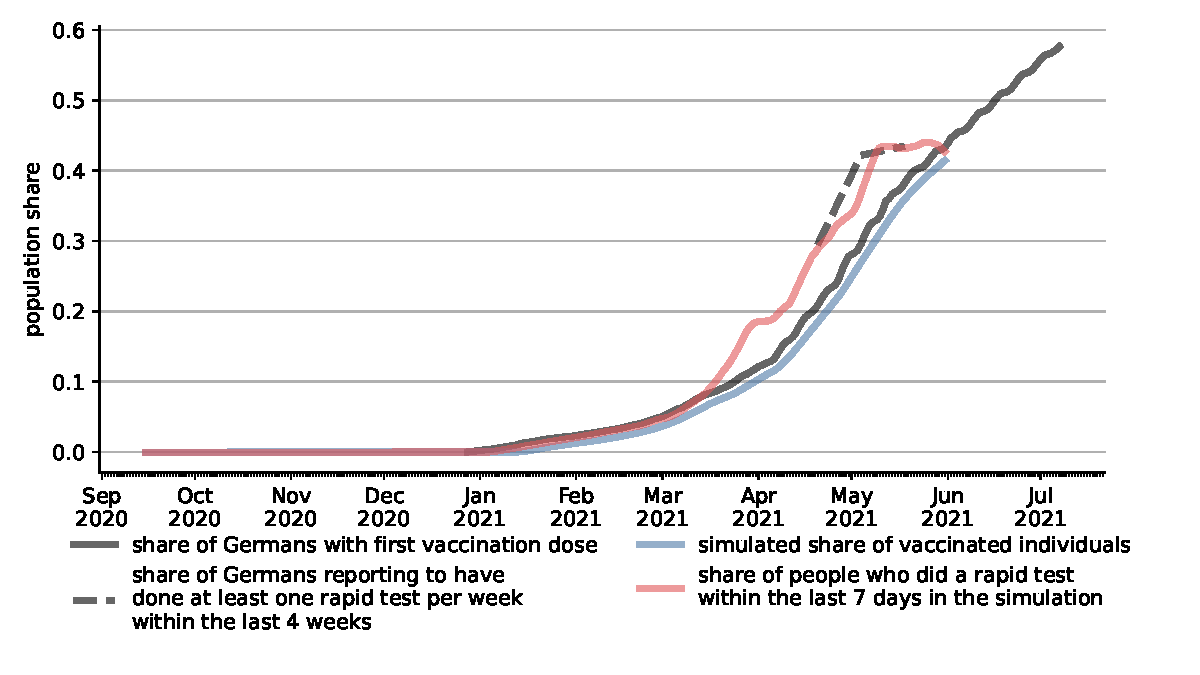
\includegraphics[width=\textwidth]{figures/results/figures/scenario_comparisons/combined_fit/full_share_rapid_test_in_last_week_and_vaccinated}

        \caption{{Tests and vaccinations}}
        \label{fig:antigen_tests_vaccinations}
    \end{subfigure}

    \caption{Evolution of the pandemic, its drivers, and model fit, September 2020 to May 2021}
    \label{fig:pandemic_drivers_model_fit}

    \floatfoot{\noindent \textit{Note:} Data sources are described in Supplementary
        Material~\ref{sec:materials_and_methods}. Age- and region-specific analogues to
        Figure~\ref{fig:aggregated_fit} can be found in Supplementary Material
        \ref{subsec:fit_results}. For legibility reasons, all lines in
        Figure~\ref{fig:stringency_infectious_contacts} are rolling 7-day averages. The
        Oxford Response Stringency Index is scaled as $2 \cdot (1 -  x / 100)$, so that
        a value of one refers to the situation at the start of our sample period and
        zero means that all NPIs included in the index are turned on. The other lines in
        Figure~\ref{fig:stringency_infectious_contacts} show the product of the effect
        of contact reductions, increased hygiene regulations, and seasonality. See
        Appendix~\ref{subsec:policies} for separate plots of the three factors by
        contact type.}
\end{figure}

By March 2021, the set of policy instruments had become much more diverse. Around the
turn of the year, the first people were vaccinated with a focus on older age groups and
medical staff (Figure~\ref{fig:antigen_tests_vaccinations}). Until the end of May, 43\%
had received at least one dose of a vaccine. In late 2020, rapid tests started to
replace regular PCR tests for staff in many medical and nursing facilities. These had to
be administered by medical doctors or in pharmacies. At-home tests approved by
authorities became available in mid-March. Rapid test centers were opened, and one test
per person and week was made available free of charge. In several states, customers were
only allowed to enter certain stores with a recent negative rapid test result. These
developments are characteristic of many countries: The initial focus on NPIs to slow the
spread of the disease has been accompanied by vaccines and a growing acceptance and use
of rapid tests. At broadly similar points in time, novel strains of the virus have
started to pose additional challenges.

\section{Results}

We draw simulated samples of agents from the population structure in September 2020 and
use the model to predict recorded infection rates until the end of May 2021. See
Supplementary Materials~\ref{subsec:synthetic_population} and
\ref{sub:initial_conditions} for details. The blue line in
Figure~\ref{fig:aggregated_fit} shows that our model's predictions are very close to
officially recorded cases in the aggregate. This is also true for infections by age and
geographical region (see Supplementary Material~\ref{subsec:fit_results}).

The effects of various mechanisms can be disentangled due to the distinct temporal
variation in the drivers of the pandemic. Next to the stringency index, the three lines
in Figure~\ref{fig:stringency_infectious_contacts} summarize how contact reductions,
increased hygiene regulations, and seasonality evolved since early September for each of
the three broad contact networks. For example, a value of 0.75 for the work multiplier
means that if the environment was the same as in September (levels of infection rates,
no rapid tests or vaccinations, only the wildtype virus present), infections at the
workplace would be reduced by 25\%. Two aspects are particularly interesting. First, all
lines broadly follow the stringency index and they would do so even more if we left out
seasonality and school vacations (roughly the last two weeks of October, two weeks each
around Christmas and Easter, and some days in late May). Second, the most stringent
regulations coincide with the period of decreasing infection rates between late December
2020 and mid-February 2021. The subsequent reversal of the trend is associated with the
spread of the B.1.1.7 variant. During the steep drop in recorded cases during May 2021,
for 42\% of the population took at least one rapid tests per week, the first-dose
vaccination rate rose from 28\% to 43\%, and seasonality lowered the relative
infectiousness of contacts.

In order to better understand the contributions of rapid tests, vaccinations, and
seasonality on the evolution of infections in 2021,
Figure~\ref{fig:2021_scenarios_broad} considers various scenarios. NPIs are always held
constant at their values in the baseline scenario.
Figure~\ref{fig:2021_scenarios_recorded} shows the model fit (the blue line, same as in
Figure~\ref{fig:aggregated_fit}), a scenario without any of the three factors (red
line), and three scenarios turning each of these factors on individually.
Figure~\ref{fig:2021_scenarios_newly_infected} does the same for total infections in the
model. Figure~\ref{fig:2021_scenarios_decomposition} employs Shapley values
\citep{Shapley2016} to decompose the difference in total infections between the scenario
without any of the three factors and our main specification.

\begin{figure}[!tp]
    \centering

    \begin{subfigure}[b]{0.475\textwidth}
        \centering
        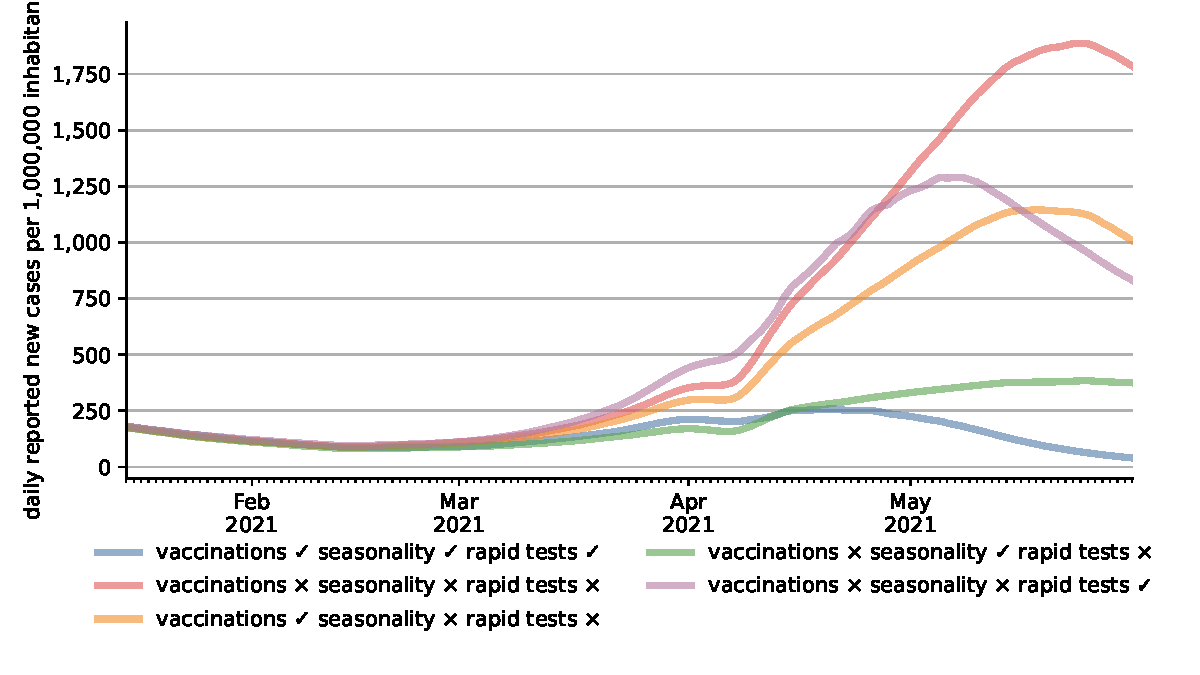
\includegraphics[width=\textwidth]{figures/results/figures/scenario_comparisons/effect_of_channels_on_pessimistic_scenario/full_new_known_case}
        \caption{{Recorded cases: 2021 scenarios}}
        \label{fig:2021_scenarios_recorded}
    \end{subfigure}
    \hfill
    \begin{subfigure}[b]{0.475\textwidth}
        \centering
        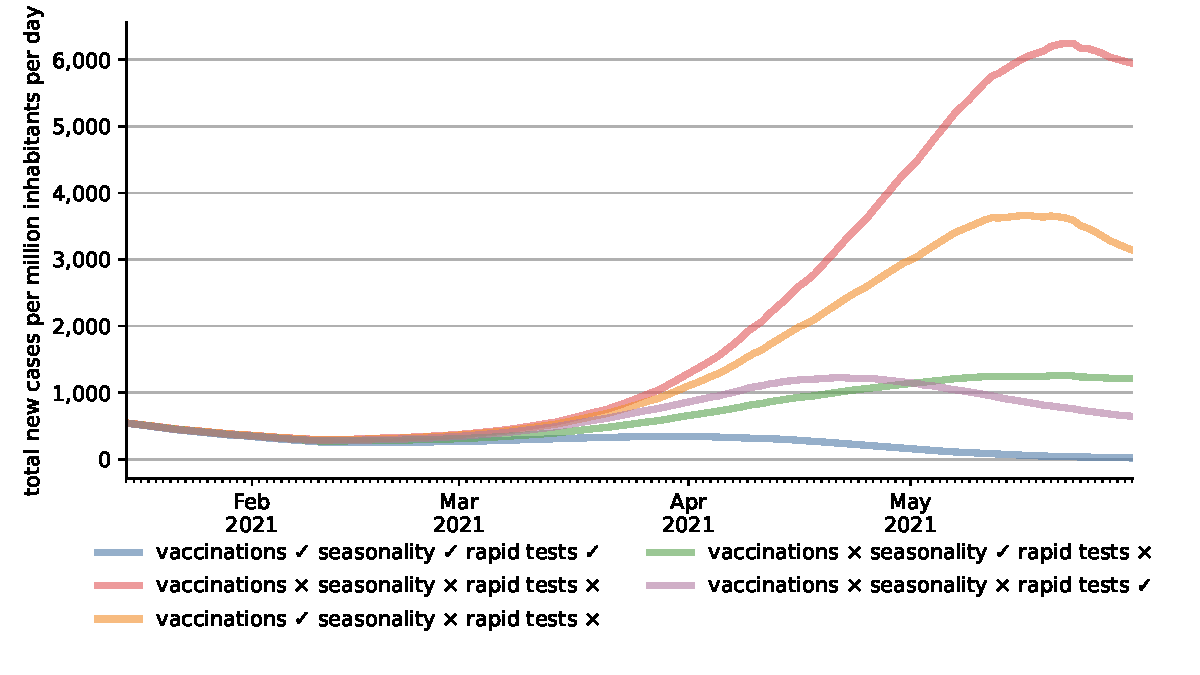
\includegraphics[width=\textwidth]{figures/results/figures/scenario_comparisons/effect_of_channels_on_pessimistic_scenario/full_newly_infected}
        \caption{{Total cases: 2021 scenarios}}
        \label{fig:2021_scenarios_newly_infected}
    \end{subfigure}

    \begin{subfigure}[b]{0.475\textwidth}
        \centering
        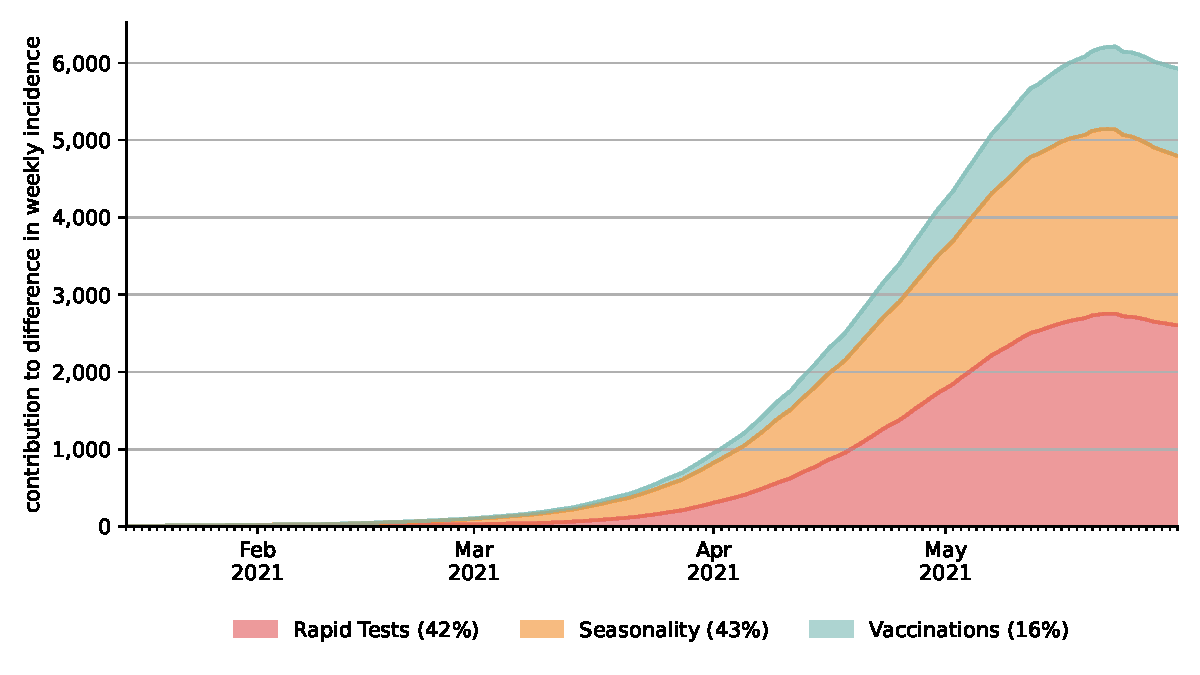
\includegraphics[width=\textwidth]{figures/results/figures/full_decomposition_channels_area}
        \caption{Decomposition of the difference between the scenario without any of the
            three factors and the main scenario in
            Figure~\ref{fig:2021_scenarios_newly_infected}.}
        \label{fig:2021_scenarios_decomposition}
    \end{subfigure}
    \hfill
    \begin{subfigure}[b]{0.475\textwidth}
        \centering
        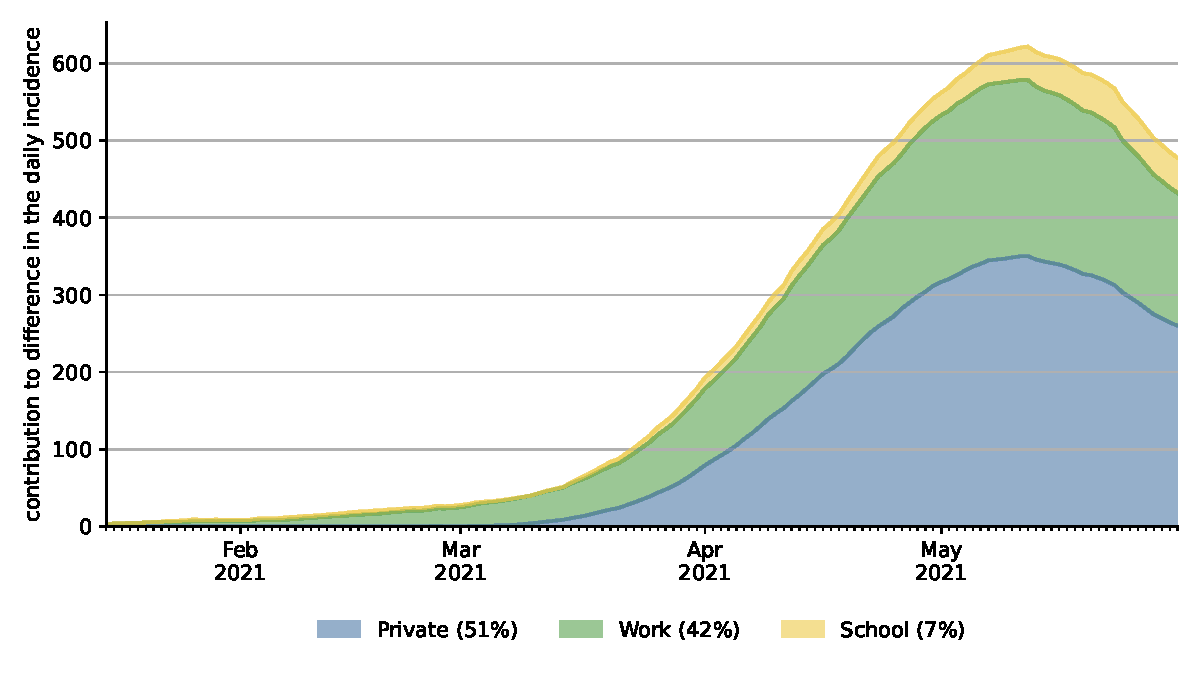
\includegraphics[width=\textwidth]{figures/results/figures/full_decomposition_rapid_tests_area}
        \caption{Decomposition of the difference between the scenario without rapid
            tests and the main scenario in
            Figure~\ref{fig:2021_scenarios_newly_infected}.}
        \label{fig:2021_scenarios_decomposition_tests}
    \end{subfigure}

    \caption{The effect of different interventions on recorded and actual infections}
    \label{fig:2021_scenarios_broad}

    \floatfoot{\noindent \textit{Note:} The blue line in
        Figure~\ref{fig:2021_scenarios_recorded} is the same as in
        Figure~\ref{fig:aggregated_fit} and refers to our baseline scenario, so does the
        blue line in Figure~\ref{fig:2021_scenarios_newly_infected}. The red lines refer
        to a situation where NPIs evolve as in the baseline scenario and the B.1.1.7
        variant is introduced in the same way; vaccinations, rapid tests, and
        seasonality remain at their January levels. The other scenarios turn each of
        these three factors on individually. The decompositions in
        Figures~\ref{fig:2021_scenarios_decomposition} and
        \ref{fig:2021_scenarios_decomposition_tests} are based on Shapley values, which
        are explained more thoroughly in Appendix~\ref{sub:shapley_value}. For
        legibility reasons, all lines are rolling 7-day averages.}
\end{figure}

Until mid-March, there is no visible difference between the different scenarios.
Seasonality hardly changes, and only few vaccinations and rapid tests were administered.
Even thereafter, the effect of the vaccination campaign is surprisingly small at first
sight. Whether considering recorded or total infections with only one channel active,
the final level is always the highest in case of the vaccination campaign (orange
lines). The Shapley value decomposition shows that vaccinations contribute 16\% to the
cumulative difference between scenarios. Reasons for the low share are the slow
start---it took until March~24th until 10\% of the population had received their first
vaccination, the 20\% mark was reached on April 19th---and the focus on older
individuals. These groups contribute less to the spread of the disease than others due
to a lower number of contacts. By the end of our study period, when first-dose
vaccination rates reached 43\% of the population, the numbers of new cases would have
started to decline. It is important to note that the initial focus of the campaign was
to prevent deaths and severe disease. Indeed, the case fatality rate was considerably
lower during the third wave when compared to the second (4.4\% between October and
February and 1.4\% between March and the end of May).

Seasonality has a large effect in slowing the spread of SARS-CoV-2. By May 31, both
observed and total cases would be reduced by a factor of four if only seasonality
mattered. However, in this period, cases would have kept on rising throughout, just at a
much lower pace \citep[this is in line with results in][, which our seasonality measure
    is based on]{Gavenciak2021}. Nevertheless, we estimate seasonality to be a
quantitatively important factor determining the evolution of the pandemic, explaining
most of the early changes and 43\% of the cumulative difference by the end of May.

A similar-sized effect---42\% in the decomposition---comes from rapid testing. Here, it
is crucial to differentiate between recorded cases and actual cases. Additional testing
means that additional infections will be recorded which would otherwise remain
undetected. Figure~\ref{fig:2021_scenarios_recorded} shows that this effect is large and
may persist for some time. Until late April, recorded cases are higher in the scenario
with rapid testing alone when compared to the setting where none of the three mechanisms
are turned on. The effect on total cases, however, is visible immediately in
Figure~\ref{fig:2021_scenarios_newly_infected}. Despite the fact that only 10\% of the
population performed weekly rapid tests in March on average, new infections on April~1
would have been reduced by 53\% relative to the scenario without vaccinations, rapid
tests, or seasonality. \label{r.1.b}\Copy{r.1.b}{In
    Appendix~\ref{subsec:robustness_rapid_test_sensitivity}, we provide a detailed analysis
    of whether our results are robust regarding the sensitivity parameters we assume for
    rapid tests. Even if we take a pessimistic stance, the effect is only reduced from 42\%
    to 38\%.}

So why is rapid testing so effective? In order to shed more light on this question,
Figure~\ref{fig:2021_scenarios_decomposition_tests} decomposes the difference in the
scenario without rapid tests and the main specification into the three channels for
rapid tests. Tests at schools have the smallest effect, which is largely explained by
schools not operating at full capacity during our period of study and the relatively
small number of students.\footnote{18\% of our population are in the education sector
    (pupils, teachers, etc.); 46\% are workers outside the education sector.} Almost 40\%
come from tests at the workplace. Despite the fact that rapid tests for private reasons
are phased in only in mid-March, they make up for more than half of the total effect.
The reason lies in the fact that a substantial share of these tests is driven by an
elevated probability to carry the virus, i.e., showing symptoms of CoViD-19 or following
up on a positive test of a household member. The latter is essentially a form of contact
tracing, which has been shown to be very effective \citep{Contreras2021,
    Fetzer2021,Kretzschmar2020}. Indeed, a deeper analysis in Supplementary
Material~\ref{subsec:appendix_scenarios} shows that the same amount of rapid tests
administered randomly in the population would not have been nearly as effective.


\section{Discussion and conclusions}

Having quantified the effects of various mechanisms, we now simulate hypothetical
scenarios comparing changes in NPIs and testing regimes. Two of the most contentious
NPIs concern schools and mandates to work from home.\label{ref.2.a} In many countries,
schools switched to remote instruction during the first wave, so did Germany. After the
summer break, they were operating at full capacity with increased hygiene measures,
before being closed again from mid-December onward. Some states started opening them
gradually in late February, but operation at normal capacity did not resume until the
beginning of June. Figure~\ref{fig:school_scenarios} shows the effects of different
policies regarding schools starting after Easter, at which point rapid tests had become
widely available. We estimate the realized scenario to have essentially the same effect
as a situation with closed schools. Under fully opened schools with mandatory tests,
total infections would have been 6\% higher; this number rises to 20\% without tests.
These effect sizes are broadly in line with empirical studies (e.g. \citet{Vlachos2021,
    Berger2021}, see Section~\ref{subsec:model_validation} for a comparison). In light of
the large negative effects school closures have on children and parents
\citep{Luijten2021, Melegari2021}---and in particular on those with low socio-economic
status---these results in conjunction with hindsight bias suggest that opening schools
combined with a testing strategy would have been beneficial. In other situations, and
particular when rapid test are not available at scale, trade-offs may well be different.

\begin{figure}[!tp]
    \centering

    \begin{subfigure}[b]{0.425\textwidth}
        \centering
        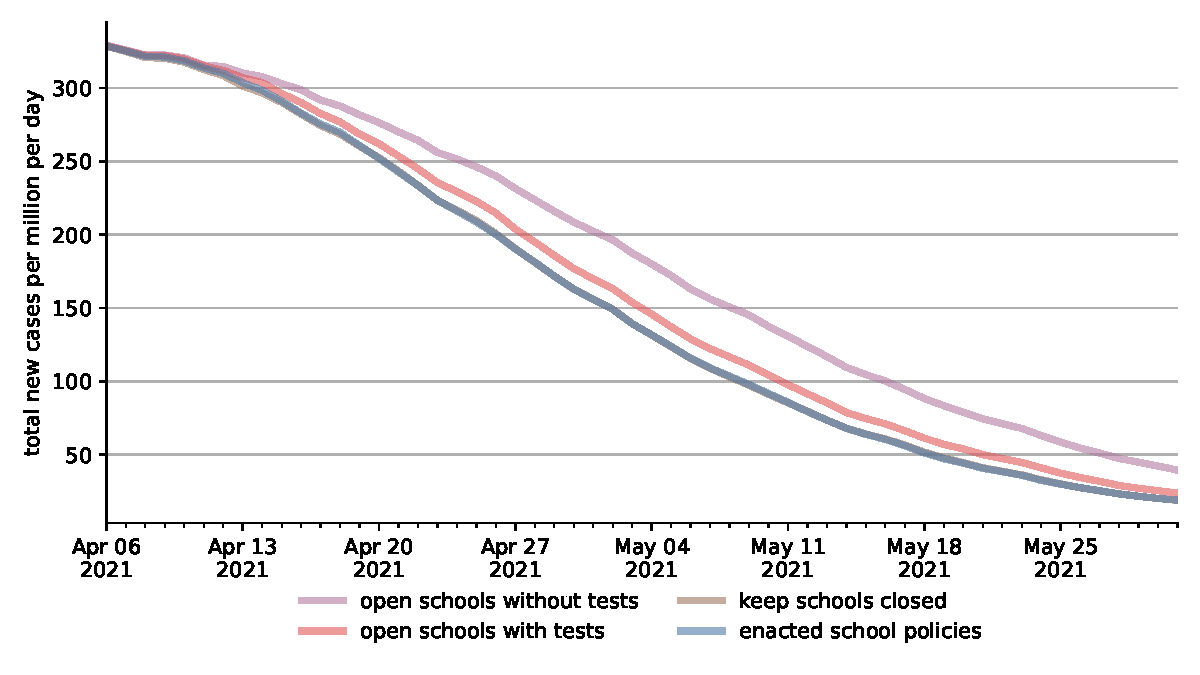
\includegraphics[width=\textwidth]{figures/results/figures/scenario_comparisons/school_scenarios/full_newly_infected}
        \caption{{Effects of different schooling scenarios}}
        \label{fig:school_scenarios}
    \end{subfigure}
    \hfill
    \begin{subfigure}[b]{0.425\textwidth}
        \centering
        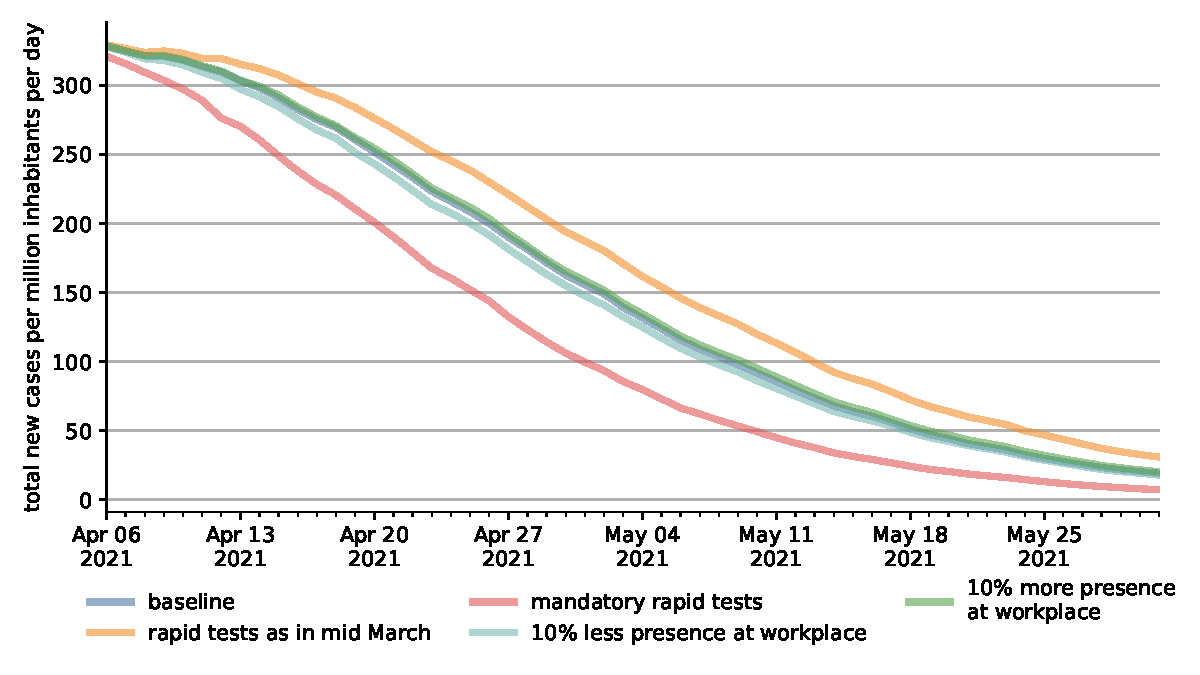
\includegraphics[width=\textwidth]{figures/results/figures/scenario_comparisons/new_work_scenarios/full_newly_infected}
        \caption{{Effects of different work scenarios}}
        \label{fig:workplace_scenarios}
    \end{subfigure}
    \vskip3ex

    \caption{Effects of different scenarios for policies regarding schools and workplaces.}
    \label{fig:school_workplace_scenarios}

    \floatfoot{\noindent \textit{Note:} Blue lines in both figures refer to our baseline
        scenario; they are the same as in
        Figure~\ref{fig:2021_scenarios_newly_infected}. Interventions start at Easter
        because there were no capacity constraints for rapid tests afterwards. For
        legibility reasons, all lines are rolling 7-day averages.}

\end{figure}

Figure~\ref{fig:workplace_scenarios} shows that with a large fraction of workers
receiving tests, testing at the workplace has larger effects than mandating employees to
work from home. Whether the share of workers working at the usual workplace is reduced
or increased by ten percent changes infection rates by 2.5\% or less in either
direction. Making testing mandatory twice a week---assuming independent compliance by
employers and workers of 95\% each---would have reduced infections by 23\%. Reducing
rapid tests offers by employers to the level of March would have increased infections by
13\%.

Our analysis has shown that during the transition to high levels of vaccination and
possibly thereafter, large-scale rapid testing can substitute for some NPIs. This comes
at a fraction of the cost. A week of the fairly strict lockdown in early 2021 is
estimated to have cost around 50~Euros per capita \citep{Wollmershauser2021}; retail
prices for rapid tests were below one Euro in early June 2021 and below five Euros for
firms. While we do not distinguish between self-administered rapid tests and point of
care rapid tests, the former are likely to play a larger role for indication-driven
testing. Widespread availability at low prices seems important. However, they rely on
purely voluntary participation in a non-public setting. The benefit of point-of-care
rapid tests as a precondition to participate in leisure activities as well as mandatory
tests at the workplace or at school come from screening the entire population. This is
important because disadvantaged groups are less likely to be reached by testing
campaigns relying on voluntary participation \citep[e.g.][]{StillmanTonin2021}; at the
same time, these groups have a higher risk to contract CoViD-19
\citep{KochInstitut2021a}. Mandatory tests at school and at the workplace will extend
more into these groups. The same goes for individuals who exhibit a low level of
compliance with CoViD-19-related regulations. Compared to vaccinations, rapid testing
programmes allow a much quicker roll-out, making it arguably the most effective tool to
contain the pandemic in the short run.
